\section{Background}
In this section we give a brief overview of the Dissent messaging system, and the deployment model adopted by Verdict, which builds on Dissent.

\subsection{Dissent messaging protocol}
A Dissent group is a closed group of pre-registered nodes. All members of the group run the Dissent protocol, which is executed in rounds. Each round of the protocol consists of two stages - shuffle stage and bulk transfer stage. The shuffle stage can be initiated by a member internal or external to the group, and each member sends a message of fixed length to the protocol. The protocol determines the transmission slot for each member by generating a random permutation of the messages sent by the members. Each member learns its own slot of transmission, but it cannot determine the nodes that will be transmitting in other slots. The bulk transfer stage involves transmission of the actual message from the member owning the slot. %In order to prevent traffic analysis attacks, rest of the group members transmit a dummy message in the phase.

\subsection{Deployment model}
\begin{figure*}
\centering
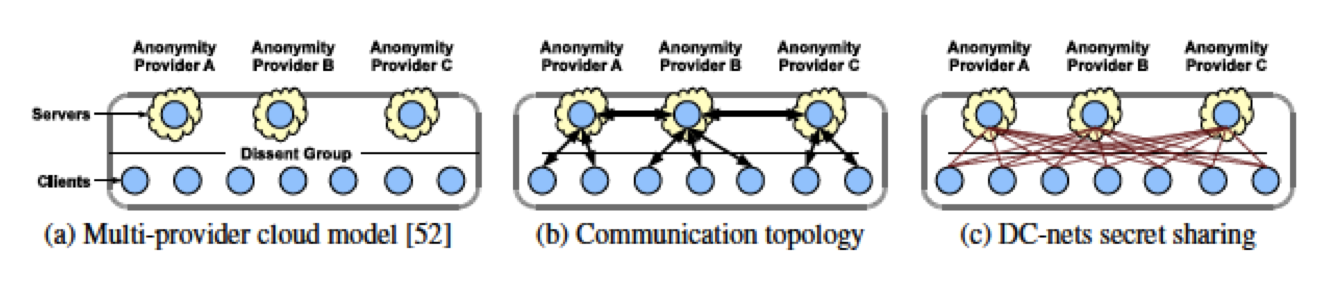
\includegraphics[width=0.7\linewidth]{dissent-model}
\caption{Verdict deployment model}
\label{fig:dissent-model}
\end{figure*}

Verdict, another anonymous messaging system adopts the Dissent protocol in a multi-server cloud deployment model with small number of unreliable clients and few highly available servers. The system follows \emph{anytrust model}, meaning the clients need trust only one server in the group. The clients share a secret with each server, which prevents any single server from deciphering the encrypted message without cooperation from all other servers.

As shown in figure \ref{fig:dissent-model}, the cloud model enables the clients to directly communicate with one or more upstream servers, without waiting for the availability of other clients in the group. In practice, there is a tradeoff between the anonymity of clients participating in the protocol execution and the threat of an individual malicious client causing a denial-of-service attack by making all the servers wait to receive a message from it.

The servers carry the computation and communication burden of the protocol by exchanging the client ciphertexts with all the other servers. The protocol runs in several stages, as follows - (i) Each client computes a ciphertext over its message using a shared secret with each server in the group. If the client owns the transmission slot (as determined using the shuffle protocol), it sends its message, otherwise it sends a dummy message. (ii) The servers collect the ciphertexts from their connected downstream clients, and forward their set to all the other servers. (iii) The servers then generate a server ciphertext corresponding to the set of clients participating in the round and exchange them with each other. (iv) Finally, the servers can combine the client ciphertexts and the server ciphertexts to reveal the plaintext message transmitted in that round and forward the signed message back to the clients downstream.

Since the Verdict protocol uses zero-knowledge proofs for verifying correctness of transmitted ciphertexts, the computation costs of the protocol can be pretty high.

In a group of size $N$, the shuffle phase requires serial communication among the nodes and incurs a startup latency of $O(N^3)$. The bulk phase involve data transmission, which is fully parallelizable and incurs a latency of $O(N^3) + O(L)$, where $L$ is the length of the message to be transmitted.

Because of these costs, the performance of the Dissent and Verdict protocols does not scale beyond a small group of nodes (see figure \ref{fig:dissent-verdict-perf}).

\begin{figure}
\centering
\includegraphics[width=0.9\linewidth]{dissent-verdict-perf}
\caption{Costs of shuffle and message transmission stages in Dissent and Verdict}
\label{fig:dissent-verdict-perf}
\end{figure}

%If each node i sends a message $m_i$ of length $L_i$, the length of the output is $\Sigma{L_i}$. This phase involves serial communication among the members, which leads to a latency of $O(N^2L)$, where $N$ is the size of the group and L is the length of the messages.